\documentclass[a4paper,14pt]{article}

\usepackage{comment} % Para comentar várias linhas ao mesmo tempo

%matemática
\usepackage{amsmath}
\usepackage{amssymb}

%diagramação
\usepackage{extsizes}
\everymath{\displaystyle}
\usepackage{geometry}
\usepackage{fancyhdr}
\usepackage{multicol}
\usepackage{graphicx}
\usepackage[brazil]{babel}
\usepackage[shortlabels]{enumitem}
\usepackage{cancel}
\usepackage{textcomp}
\usepackage{tcolorbox}

%tabelas
\usepackage{array} % Para melhor formatação de tabelas
\usepackage{longtable}
\usepackage{booktabs}  % Para linhas horizontais mais bonitas
\usepackage{float}   % Para usar o modificador [H]
\usepackage{caption} % Para usar legendas em tabelas
\usepackage{wrapfig} % Para usar tabelas e figuras flutuantes
\usepackage{xcolor} % Para cores do fundo de tabelas
\usepackage{colortbl} % Para cores do fundo de tabelas

%tikzpicture
\begin{comment}
	\usepackage{tikz}
	\usepackage{scalerel}
	\usepackage{pict2e}
	\usepackage{tkz-euclide}
	\usetikzlibrary{calc}
	\usetikzlibrary{patterns,arrows.meta}
	\usetikzlibrary{shadows}
	\usetikzlibrary{external}
\end{comment}


%pgfplots
\usepackage{pgfplots}
\pgfplotsset{compat=newest}
\usepgfplotslibrary{statistics}
\usepgfplotslibrary{fillbetween}

%colours
\usepackage{xcolor}



\columnsep=2cm
\hoffset=0cm
\textwidth=8cm
\setlength{\columnseprule}{.1pt}
\setlength{\columnsep}{2cm}
\renewcommand{\headrulewidth}{0pt}
\geometry{top=1in, bottom=1in, left=0.7in, right=0.5in}

\pagestyle{fancy}
\fancyhf{}
\fancyfoot[C]{\thepage}

\begin{document}
	
	\noindent\textbf{6FMA124, 6FMA125 - Matemática} 
	
	\begin{center}Exercícios de triângulos (Versão estudante)
	\end{center}
	
	\noindent\textbf{Nome:} \underline{\hspace{10cm}}
	\noindent\textbf{Data:} \underline{\hspace{4cm}}
	
	%\section*{Questões de Matemática}
	
	\begin{multicols}{2}
	    \noindent \begin{itemize}
	    	\item Casos de congruência: LAL, LLL e ALA.
	    	\item A soma dos ângulos internos de um triângulo é 180°.
	    	\item Podemos classificar os triângulos de dois modos diferentes, de acordo com as características de seus lados ou de seus ângulos. Observe:
	    \end{itemize}
	    \textbf{Caracterização dos lados}
	    \begin{itemize}
	    	\item \textbf{Equilátero:} três lados congruentes
	    	\item \textbf{Isóceles:} dois lados congruentes
	    	\item \textbf{Escaleno:} não possui nenhum par de lados congruentes.
	    \end{itemize}
	     \textbf{Caracterização dos ângulos}
	    \begin{itemize}
	    	\item \textbf{Retângulo:} um ângulo reto.
	    	\item \textbf{Obtusângulo:} um ângulo obtuso.
	    	\item \textbf{Acutângulo:} todos os ângulos agudos.
	    \end{itemize}
		\noindent\textsubscript{--------------------------------------------------------------------------}
		\begin{enumerate} 
			\columnbreak
			\item Desenhe o triângulo cujos lados menores são perpendiculares e medem 6 cm cada um. Qual é a medida do lado maior? \\\\\\\\\\\\\\\\\\\\\\\\
			\item No desenho a seguir, são dados um lado de um triângulo e os ângulos adjacentes a ele. Desenhe o triângulo e apresente a medida do terceiro ângulo. \\\\\\\\\\\\\\
			Compare o seu triângulo com os dos seus colegas. Eles são congruentes. Por quê? \\\\\\\\\
			\item Determine o valor de $x$ (medida de comprimento ou de ângulo) nos triângulos a seguir. \\
			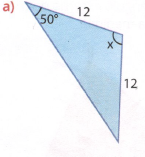
\includegraphics[width=1\linewidth]{6FMA124_imagens/imagem1}
			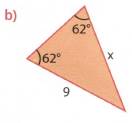
\includegraphics[width=1\linewidth]{6FMA124_imagens/imagem2}
			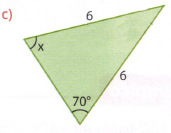
\includegraphics[width=1\linewidth]{6FMA124_imagens/imagem3}
			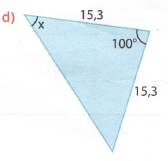
\includegraphics[width=1\linewidth]{6FMA124_imagens/imagem4}
			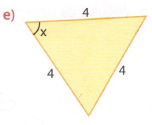
\includegraphics[width=1\linewidth]{6FMA124_imagens/imagem5}
			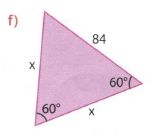
\includegraphics[width=1\linewidth]{6FMA124_imagens/imagem6}
			\item Triângulos equiláteros também são isósceles? E os triângulos isósceles são equiláteros? \\\\\\\\
			\item Num triângulo isósceles, os ângulos da base medem 26°. Qual é a medida do maior ângulo? \\\\\\\\\\\\\\\\\\\\\\\\\\\\\\
			\item Num triângulo isósceles, um ângulo mede 96°. Quais são as medidas dos demais ângulos? \\\\\\\\\\\\\\\\\\\\\\\\\\\\\\\\\\\\
			\item A medida de um ângulo externo de um triângulo é igual a soma das medidas dos ângulos internos não adjacentes a ele. Sendo $\theta$ um ângulo externo do triângulo ABC abaixo, determine sua medida. \\
			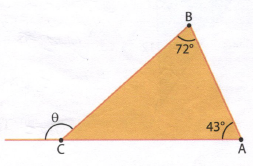
\includegraphics[width=1\linewidth]{6FMA124_imagens/imagem7} \\\\\\\\\\\\\\\\\\
			\textbf{Desafio olímpico} \\\\
			(OBMEP) No triângulo $ABC$, temos $AB = AC$ e os cinco segmentos marcados têm todos a mesma medida. Qual é a medida do ângulo $B$$\hat{A}C$? \\
			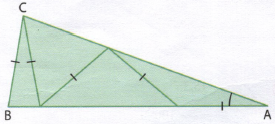
\includegraphics[width=1\linewidth]{6FMA124_imagens/imagem8}
			\begin{enumerate}[a)]
				\item 10°
				\item 15°
				\item 20°
				\item 25°
				\item 30°
			\end{enumerate}
			%54 a 66
			\item Desenhe, com régua e compasso, um triângulo retângulo isósceles, cujos catetos medem 6 cm. \\\\\\\\\\\\\\\\\\\\\\\\\\\\\\\\
			\item Você deve se lembrar que, numa pirâmide regular, todas as arestas laterais têm a mesma medida e as arestas da base são congruentes. Na pirâmide regular de base triangulas representada ao lado, sabe-se que $VA = 92$ cm e $AC = 92$ cm. Complete: \\
			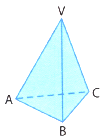
\includegraphics[width=0.5\linewidth]{6FMA124_imagens/imagem9}
			\begin{enumerate}[a)]
				\item $VB = $ ..... cm
				\item $AB = $ ..... cm
				\item $BC = $ ..... cm
				\item $m (V\hat{A}B) = $ ..... °
				\item $m (B\hat{V}C) = $ ..... °
				\item $\Delta$$VAB \cong \Delta$$ABC$, pelo caso LLL. Essa afirmação é ..... . (V ou F)
				\item $\Delta$$VAB \cong \Delta$$VBC$, pelo caso LLL. Essa afirmação é ..... . (V ou F)
			\end{enumerate}
			\item Num triângulo isósceles, cada um dos ângulos da base mede o quádruplo do outro ângulo. Quanto medem os ângulos da base? \\\\\\\\\\\\\\\\
			\item Seja $ABC$ um triângulo isósceles de base $\overline{BC}$. Sejam $M$ e $N$ os pontos médios de $\overline{AB}$ e $\overline{AC}$, respectivamente. Mostre que as medianas $\overline{BN}$ e $\overline{CM}$ são congruentes. (Uma mediana de um triângulo é um segmento que liga um vértice do triângulo ao ponto médio do lado oposto.) \newpage
			\item Sabe-se que todo ponto pertencente à mediatriz de um segmento é equidistante às extremidades do segmento. Será que existe algum ponto que não pertence à mediatriz e tem a mesma propriedade? Vamos demonstrar que a resposta a essa pergunta é \textbf{não}.
			\begin{enumerate}[a)]
				\item Seja $\overline{AB}$ um segmento de $M$, o seu ponto médio. Considere um ponto $X$ equidistante a $A$ e $B$, ou seja, tal que $XA = XB$. Mostre que $\Delta$$AMX \cong \Delta$$BMX$, justificando sua prova. \\\\\\\\\\\\\\
				\item Qual é o ângulo formado pelas retas $\overleftrightarrow{AB}$ e $\overleftrightarrow{XM}$? \\\\\\\\\\\\
				\item Conclua que $X$ deve pertencer à mediatriz de $\overline{AB}$. \\\\\\\\\\\\
			\end{enumerate}
			\item Sabendo da propriedade qua as mediatrizes têm, mostre o que você tinha conjecturado: as mediatrizes dos lados de um triângulo encontram-se em um ponto. \\\\\\\\\\\\\\\\\\
			\item Na figura a seguir, $ABCD$ e $EFGH$ são quadrados. \\
			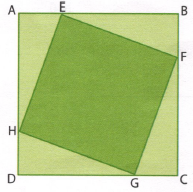
\includegraphics[width=1\linewidth]{6FMA124_imagens/imagem10}
			Mostre que $\Delta$$AEH \cong \Delta$$DHG$. \newpage
			\item Na figura plana $ABCD$, representada a seguir, temos $AB = DC$ e $AD = BC$. Prove que $\hat{A} \cong \hat{C}$ e $\hat{B} \cong \hat{D}$. \\
			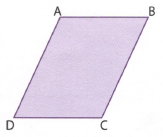
\includegraphics[width=1\linewidth]{6FMA124_imagens/imagem11} \\\\\\\\\\\\\\\\\\\\\\\\
			\item Um dos ângulos de um triângulo mede 46°. Sabendo que esse triângulo é isósceles, qual a maior medida que um ângulo interno do triângulo pode ter? \\\\\\\\\\\\\\\\\\
			\item Num triângulo isósceles, um dos ângulos mede 130°. Quanto medem os demais ângulos? \\\\\\\\\\\\\\\\\\
			\item Vamos mostrar mais um cado de congruência de triângulos: o caso LAA$_O$ (lado, ângulo, ângulo oposto). Observe as figuras: \\
			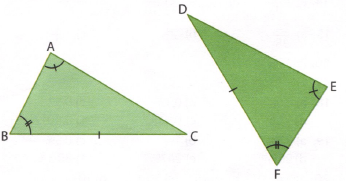
\includegraphics[width=1\linewidth]{6FMA124_imagens/imagem12}
			Mostre que $\hat{C} \cong \hat{D}$ e conclua que $\Delta$$ABC \cong \Delta$$EFD$. \newpage
			\item Construa, com régua e compasso, um triângulo de lados 7, 8 e 9 cm. Em seguida, ainda com régua e compasso, trace as mediatrizes dos lados. O que parece acontecer? \\\\\\\\\\\\\\\\\\\\\\\\\\\\\\\\\\\\\\\\\\\\\\\\\\\\\\\\\\\\\\\\\\\\\\
			\item Será que, se dois triângulos têm dois pares de lados respectivamente congruentes e um par de ângulos que não são os que estão entre os lados em questão, então eles são congruentes? Em outras palavras, será que existe o caso LLA$_O$ (lado, lado, ângulo oposto)?  \\
			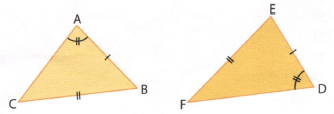
\includegraphics[width=1\linewidth]{6FMA124_imagens/imagem13}
			Veremos que a resposta para essa pergunta é \textbf{não}.
			Por isso, tome muito cuidado para não errar e ser enganado pelo falso caso LLA$_O$! \\
			Desenhe, com régua e compasso, dois triângulos não congruentes $ABC$ e $DEF$, sabendo que $AB = DE = 8 cm, BC = EF = 7$ cm e $m(\hat{A}) = m(\hat{D}) = 45\circ$.
		\end{enumerate}
		$~$ \\ $~$ \\ $~$ \\ $~$ \\ $~$ \\ $~$ \\ $~$ \\ $~$ \\ $~$ \\ $~$ \\ $~$ \\ $~$ \\ $~$ \\ $~$ \\ $~$ \\ $~$ \\ $~$ \\ $~$
	\end{multicols}
\end{document}